%% LyX 2.3.4.2 created this file.  For more info, see http://www.lyx.org/.
%% Do not edit unless you really know what you are doing.
\documentclass[english,dvipsnames,aspectratio=169,handout]{beamer}
\usepackage{xcolor}

\usepackage{mathptmx}
\usepackage{eulervm}
\usepackage[T1]{fontenc}
\usepackage[latin9]{inputenc}
\usepackage{babel}
\usepackage{amstext}
\usepackage{amssymb}
\usepackage{graphicx}
\usepackage{ifthen}
\usepackage{xcolor}
\usepackage{xspace}
\usepackage{tikz}
\usetikzlibrary{tikzmark}
\usetikzlibrary{calc}
\usepackage{pgfplots}
%\pgfplotsset{compat=1.17}
\usepackage{booktabs}
\usepackage{xpatch}
\usepackage{multirow}
\usepackage{colortbl}
\usepackage{pgfpages}

\newcommand{\commenteq}[1]{{\color{brown}#1}}
<<<<<<< HEAD
=======
% \newcommand{\alarm}[1]{{\color{red}#1}}
>>>>>>> b9da050859818a1e73d1b2e41e08fb916b05ca83



\xpatchcmd{\itemize}
  {\def\makelabel}
  {\ifnum\@itemdepth=1\relax
     \setlength\itemsep{2ex}% separation for first level
   \else
     \ifnum\@itemdepth=2\relax
       \setlength\itemsep{1ex}% separation for second level
     \else
       \ifnum\@itemdepth=3\relax
         \setlength\itemsep{0.5ex}% separation for third level
   \fi\fi\fi\def\makelabel
  }
 {}
 {}

\ifx\hypersetup\undefined
  \AtBeginDocument{%
    \hypersetup{unicode=true,pdfusetitle,
 bookmarks=true,bookmarksnumbered=false,bookmarksopen=false,
 breaklinks=false,pdfborder={0 0 0},pdfborderstyle={},backref=false,colorlinks=true,
 allcolors=NYUPurple,urlcolor=LightPurple}
  }
\else
  \hypersetup{unicode=true,pdfusetitle,
 bookmarks=true,bookmarksnumbered=false,bookmarksopen=false,
 breaklinks=false,pdfborder={0 0 0},pdfborderstyle={},backref=false,colorlinks=true,
 allcolors=NYUPurple,urlcolor=LightPurple}
\fi

\makeatletter

%%%%%%%%%%%%%%%%%%%%%%%%%%%%%% LyX specific LaTeX commands.
%% Because html converters don't know tabularnewline
\providecommand{\tabularnewline}{\\}

%%%%%%%%%%%%%%%%%%%%%%%%%%%%%% Textclass specific LaTeX commands.
% this default might be overridden by plain title style
\newcommand\makebeamertitle{\frame{\maketitle}}%
% (ERT) argument for the TOC
\AtBeginDocument{%
  \let\origtableofcontents=\tableofcontents
  \def\tableofcontents{\@ifnextchar[{\origtableofcontents}{\gobbletableofcontents}}
  \def\gobbletableofcontents#1{\origtableofcontents}
}

%%%%%%%%%%%%%%%%%%%%%%%%%%%%%% User specified LaTeX commands.
\usetheme{CambridgeUS} 
\beamertemplatenavigationsymbolsempty


% Set Color ==============================
\definecolor{NYUPurple}{RGB}{87,6,140}
\definecolor{LightPurple}{RGB}{165,11,255}


\setbeamercolor{title}{fg=NYUPurple}
\setbeamercolor{frametitle}{fg=NYUPurple}

\setbeamercolor{background canvas}{fg=NYUPurple, bg=white}
\setbeamercolor{background}{fg=black, bg=NYUPurple}

\setbeamercolor{palette primary}{fg=black, bg=gray!30!white}
\setbeamercolor{palette secondary}{fg=black, bg=gray!20!white}
\setbeamercolor{palette tertiary}{fg=gray!20!white, bg=NYUPurple}

\setbeamertemplate{headline}{}
\setbeamerfont{itemize/enumerate body}{}
\setbeamerfont{itemize/enumerate subbody}{size=\normalsize}

\setbeamercolor{parttitle}{fg=NYUPurple}
\setbeamercolor{sectiontitle}{fg=NYUPurple}
\setbeamercolor{sectionname}{fg=NYUPurple}
\setbeamercolor{section page}{fg=NYUPurple}
%\setbeamercolor{description item}{fg=NYUPurple}
%\setbeamercolor{block title}{fg=NYUPurple}

\setbeamertemplate{blocks}[rounded][shadow=false]
\setbeamercolor{block body}{bg=normal text.bg!90!NYUPurple}
\setbeamercolor{block title}{bg=NYUPurple!30, fg=NYUPurple}



\AtBeginSection[]{
  \begin{frame}
  \vfill
  \centering
\setbeamercolor{section title}{fg=NYUPurple}
 \begin{beamercolorbox}[sep=8pt,center,shadow=true,rounded=true]{title}
    \usebeamerfont{title}\usebeamercolor[fg]{title}\insertsectionhead\par%
  \end{beamercolorbox}
  \vfill
  \end{frame}
}

\makeatother

\setlength{\parskip}{\medskipamount} 

\input ../macros

\begin{document}
\input ../rosenberg-macros

%\setbeameroption{show notes on second screen}

\title[DS-GA 1003]{Gradient Boosting}
\author{Ravid Shwartz Ziv \\
Slides based on Lecture
\href{https://github.com/davidrosenberg/mlcourse/blob/gh-pages/Lectures/11c.gradient-boosting.pdf}{11c} from David Rosenberg's course materials (\url{https://github.com/davidrosenberg/mlcourse})
}
\date{April 11, 2023}
\institute{CDS, NYU}

\makebeamertitle
\mode<article>{Just in article version}

\begin{frame}
{Today's lecture}
\begin{itemize}
\item Another way to get non-linear models in a linear form---adaptive basis function models.
\item A general algorithm for greedy function approximation---gradient boosting machine.
    \begin{itemize}
        \item Adaboost is a special case.
    \end{itemize}
\end{itemize}
\note[item]{We've learned kernel methods which gives you a non-linear classifier in a linear form. Today we are going to learn another method called ``adaptive basis function models''.
}
\note[item]{And we are going to learn a general algorithm for learning these basis functions, which give rise to a family of boosting algorithms, including Adaboost we saw last time.}
\end{frame}

\section{Motivation}
\begin{frame}
{Recap: Adaboost}
\begin{center}
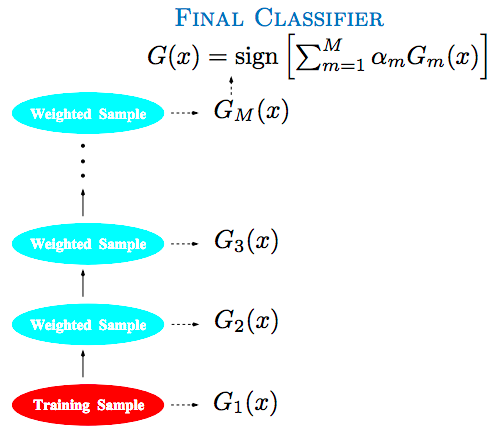
\includegraphics[height=0.7\textheight]{figures/adaboostSchematic}
\par\end{center}
\let\thefootnote\relax\footnotetext{\tiny{From ESL Figure 10.1}}
\note[item]{Recall the Adaboost algorithm we talked about last time. We want to learn a sequence of base classifiers; each of them minimizes weighted zero-one error, where the weights are higher on previously misclassified examples. It's like when you study for an exam, you go over all practice questions; then you look at the answers. The next time you spend more time on questions you go wrong. In the end you would grasp everything.}
\note[item]{Our final classifier is a weighted combination the base classifiers. The weights on good classifiers are higher, where ``good'' is measured by weighted zero-one error.}
\note[item]{Last time we went over a greedy algorithm for obtaining the base classifiers and the weights. Let's review the Adaboost algorithm.}
\end{frame}

\begin{frame}{AdaBoost: Algorithm}

Given training set $\cd=\left\{ \left(x_{1},y_{1}\right),\ldots,\left(x_{n},y_{n}\right)\right\} $.
\begin{enumerate}
\item Initialize observation weights $w_{i}=1$, $i=1,2,\ldots,n$.

\item For $m=1$ to $M$:
\begin{enumerate}
\item Base learner fits weighted training data and returns $G_{m}(x)$

\item Compute \emph{weighted empirical 0-1 risk}:
\[
\mbox{err}_{m}=\frac{1}{W}\sum_{i=1}^{n}w_{i}\ind{y_{i}\neq G_{m}(x_{i})}\quad\text{where }W=\sum_{i=1}^{n}w_{i}.
\]

\item Compute  \emph{classifier weight}: $\alpha_{m}=\ln\left(\frac{1-\text{err}_{m}}{\text{err}_{m}}\right)$.

\item Update \emph{example weight}: $w_{i}\gets w_{i}\cdot\exp\left[\alpha_{m}\ind{y_{i}\neq G_{m}(x_{i})}\right]$
\end{enumerate}
\item Return \emph{voted classifier}: $G(x)=\sign\left[\sum_{m=1}^{M}\alpha_{m}G_{m}(x)\right]$.
\onslide<+->{\hspace{2em}{\color{red}Why not learn $G(x)$ directly?}}
\end{enumerate}
%\note[item]{But why does this algorithm work? Does it actually gives us a good classifier in our hypothesis space? Let's work backwards. Since $G(x)$ is the final model we want, why don't we learn it directly? This is actually a special case of additive basis function models.}
\note[item]{Now that we have a hypothesis space, and a loss function depending on whether we are doing classification or regression, why don't we follow our familiar recipe to write down the ERM objective, and run gradient descent to learn the parameters.}
\end{frame}

\begin{frame}{Nonlinear Regression}
\begin{itemize}
\item How do we fit the following data?
\begin{figure}
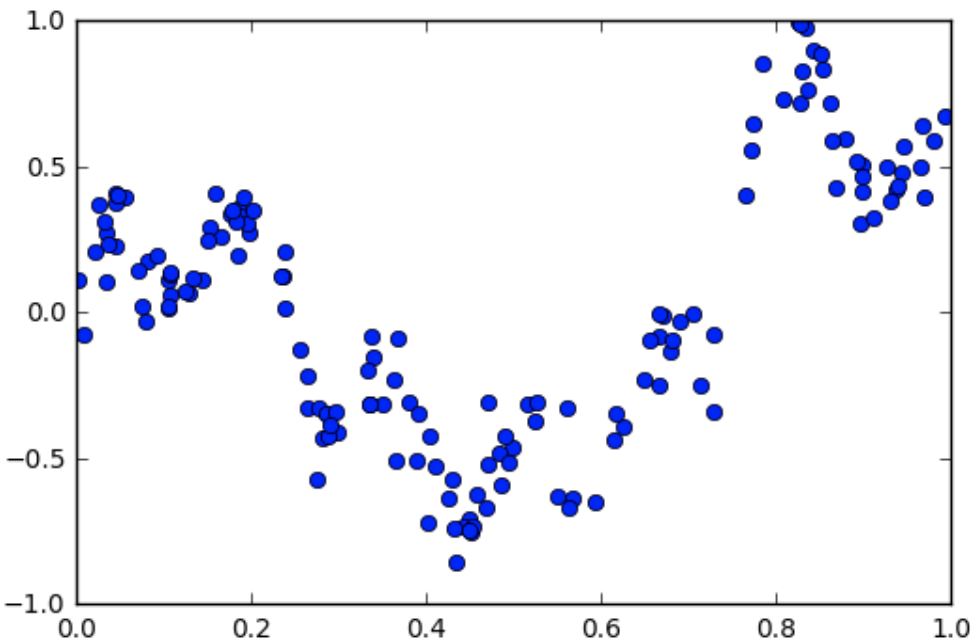
\includegraphics[height=0.6\textheight]{figures/nonlinear-regression-data}
\end{figure}
\end{itemize}
\note[item]{To motivate adaptive basis models, let's consider this nonlinear regression problem. Given the following data, what model would you use?}
\note[item]{We can create non-linear features.}
\end{frame}
%
\begin{frame}{Linear Model with Basis Functions}
\begin{itemize}[<+->]
\item Fit a linear combination of transformations of the input:
\[
f(x)=\sum_{m=1}^{M}v_{m}h_{m}(x),
\]
where $h_m$'s are called \textbf{basis functions} (or feature functions in ML):
\[
h_{1},\ldots,h_{M}:\cx\to\reals
\]
\item Example: polynomial regression where $h_m(x) = x^m$.
\item Can we use this model for classification?
\note[item]{$f(x)$ can be transformed to a probability (\eg similar to GLM), or used as a score function (\eg margin-based classification and ranking).}
\item Can fit this using standard methods for linear models (e.g. least
squares, lasso, ridge, etc.)
\begin{itemize}
\item \emph{Note that $h_m$'s are fixed and known}, \ie chosen ahead of time.
\end{itemize}
\end{itemize}
\note[item]{The key idea here is to use a family of functions or transformations that can be applied to $x$, which are called basis functions.}
\note[item]{The basis functions can be non-linear in $x$. Can you think of some examples? Polynomials, piecewise constant functions.}
\note[item]{We can use it for classification by another function to transform the results to a probability or a class, \eg sgn as in Adaboost.}
\note[item]{All inference methods we've learned for linear models can be applied here. Why? It's important to note that $h_m$ are fixed, thus they can be simply considered as another feature.}
\end{frame}
%
\begin{frame}{Adaptive Basis Function Model}
\begin{itemize}[<+->]
\item What if we want to learn the basis functions? (hence \emph{adaptive})

\item {Base hypothesis space} $\ch$ consisting of functions $h:\cx\to\reals$.

\item<.-> An \textbf{adaptive basis function expansion }over $\ch$ is
an ensemble model:
\begin{align}
f(x)=\sum_{m=1}^{M}v_{m}h_{m}(x),
\end{align}
where $v_{m}\in\reals$ and $h_{m}\in\ch$.

\item Combined hypothesis space:
\[
\cf_{M}=\left\{ \sum_{m=1}^{M}v_{m}h_{m}(x)\mid v_{m}\in\reals,\:h_{m}\in\ch,\:m=1,\ldots,M\right\} 
\]
\item<.-> What are the learnable?
\end{itemize}
\note[item]{But in Adaboost we don't know the base classifier beforehand. How to learn them?}
\note[item]{Let's formalize the problem a bit. The basis functions belong to the base hypothesis space, and our predictor is a linear combination of the basis functions, just as every vector in a vector space can be represented by a linear combination of the basis vectors.}
\note[item]{Both the weights $v_m$ and  the basis functions $h_m$ are learned, as in Adaboost.}
\end{frame}
%
%\begin{frame}{Adaptive Basis Function Model}
%\begin{itemize}
%\item \textbf{Base hypothesis space}: $\ch$ of \textbf{real-valued functions} 
%\item \textbf{Combined hypothesis space:} $\cf_{M}$:
%\[
%\cf_{M}=\left\{ \sum_{m=1}^{M}v_{m}h_{m}(x)\mid v_{m}\in\reals,\:h_{m}\in\ch,\:m=1,\ldots,M\right\} 
%\]
%
%\pause{}
%\item Suppose we're given some data $\cd=\left((x_{1},y_{1}),\ldots,(x_{n},y_{n})\right)$.
%
%\pause{}
%\item Learning is choosing $v_{1},\ldots,v_{M}\in\reals$ and $h_{1},\ldots,h_{M}\in\ch$
%to fit $\cd$.
%\end{itemize}
%\end{frame}

%\begin{frame}{Not Limited to Regression}
%\begin{itemize}
%\item Linear combination of basis functions:
%\[
%f(x)=\sum_{m=1}^{M}v_{m}g_{m}(x)
%\]
%\item $f(x)$ is a number \textemdash{} for regression, it's exactly what
%we're looking for.
%
%\pause{}
%\item Otherwise, $f(x)$ is often called a \textbf{score} function.
%\item It can be 
%\begin{itemize}
%\item thresholded to get a classification
%\item transformed to get a probability
%\item transformed to get a parameter of a probability distribution (e.g.
%Poisson regression)
%\item used for ranking search results
%\end{itemize}
%\end{itemize}
%\end{frame}
%

%
\begin{frame}{Empirical Risk Minimization}
\begin{itemize}[<+->]
\item What's our learning objective? 
\[
\hat{f}=\argmin_{f\in\cf_{M}}\frac{1}{n}\sum_{i=1}^{n}\ell\left(y_{i},f(x_{i})\right),
\]
for some {loss function} $\ell$. 

\item Write ERM objective function as
\[
J(v_{1},\ldots,v_{M},h_{1},\ldots,h_{M})=\frac{1}{n}\sum_{i=1}^{n}\ell\left(y_{i},\sum_{m=1}^{M}v_{m}h_{m}(x)\right).
\]

\item How to optimize $J$? i.e. how to learn?
\end{itemize}
\note[item]{So the main question left is how to optimize $J$. Adaboost uses a greedy algorithm. But can we directly optimize all parameters?}
\end{frame}
%
\begin{frame}{Gradient-Based Methods}
\begin{itemize}[<+->]
\item \texttt{Suppose} our base hypothesis space is parameterized by $\Theta=\reals^{b}$:
\[
J(v_{1},\ldots,v_{M},{\color{blue}\theta_{1},\ldots,\theta_{M}})=\frac{1}{n}\sum_{i=1}^{n}\ell\left(y_{i},\sum_{m=1}^{M}v_{m}h(x;{\color{blue}\theta_{m}})\right).
\]

\item Can we optimize it with SGD?
\begin{itemize}
\item Can we differentiate $J$ w.r.t. $v_{m}$'s and $\theta_{m}$'s?
\end{itemize}

\item For {some} hypothesis spaces and typical loss functions, yes!
\begin{itemize}[<.->]
\item Neural networks fall into this category! ($h_{1},\ldots,h_{M}$ are
neurons of last hidden layer.)
\end{itemize}
\end{itemize}
\note[item]{Note that $h$ doesn't have to be a parametric model; it can be non-parametric, \eg decision trees.}
\note[item]{Running SGD requires the objective to be differentiable w.r.t. the parameters, \eg neural networks.}
\end{frame}
%
\begin{frame}{What if Gradient Based Methods Don't Apply?}
\begin{simpleblock}
{{What if base hypothesis space $\ch$ consists of decision trees?}}
\begin{itemize}[<2->]
\item Can we even parameterize trees with $\Theta=\reals^{b}$?
\item Even if we could, predictions would not change continuously w.r.t. $\theta\in\Theta$, so certainly not differentiable.
\end{itemize}
\end{simpleblock}
\note[item]{First of all, we cannot really parametrize decision trees as the number of parameters depends on the tree structure. But even if we fix the tree structure, in which case the parameters are the splitting feature values, we still cannot run SGD as the function is piecewise-constant.}

\begin{simpleblock}
{\onslide<3->{What about a greedy algorithm similar to Adaboost?}}
\begin{itemize}[<4->]
\item Applies to non-parametric or non-differentiable basis functions.
\item But is it optimizing our objective using some loss function?
\end{itemize}
\end{simpleblock}
\note[item]{Adaboost gives us a model in the form of an adaptive basis function model. But what the objective function it is optimizing?}
\end{frame}

\begin{frame}
\begin{simpleblock}
{Today we'll discuss \textbf{gradient boosting}.}
\begin{itemize}
\item Gradient descent in the \emph{function space}.
\item It applies whenever 
\begin{itemize}
\item our loss function is {[}sub{]}differentiable w.r.t. training predictions
$f(x_{i})$, and
\item we can do regression with the base hypothesis space $\ch$.
\end{itemize}
\end{itemize}
\end{simpleblock}

\note[item]{Using gradient boosting, we can directly optimize the basis functions in the function space.}
\note[item]{We will show that Adaboost is just a special case of gradient boosting using the exponential loss.}
\note[item]{This algorithm is very general, it only requires...}
\end{frame}
%

\begin{frame}
{History}
\begin{table}
\begin{tabular}{rp{8cm}}
Kearns, Valiant (1989): & Can weak learners (\eg $51\%$ accuracy) be transformed to strong learners (\eg $99.9\%$ accuracy)?\pause \\
Schapire (1990) \& Freund (1995): & Yes, weak learners can be iteratively improved to a strong learner.\pause \\
Freund, Schapire (1996): & And here is a practical algorithm---Adaboost.\pause \\
Breiman (1996 \& 1998): & Yes, it works! Boosting is the best off-the-shelf classifier in the world.\pause \\
\multicolumn{2}{c}{(Attempts to explain why Adaboost works and improvements)}\pause\\
Friedman, Hastie, Tibshirani (2000): & Actually, boosting fits an additive model.\pause \\
Friedman (2001): & Furthermore, it can be considered as gradient descent in the function space.
\end{tabular}
\end{table}
    \note[item]{Adaboost is a great example where a pure theoretical investigation leads to huge practical success.}
\note[item]{The idea of boosting started from a theoretical question: can we transform weak learners that are merely better than chance to arbitrarily strong learners?}
\note[item]{Schapir and Freund first gave an affirmative answer. However their boosting algorithm at that time was mainly constructed for theoretical proofs. In 1996, Adaboost was born.}
\note[item]{There is a lot of excitement in the ML community around it. In particular, Leo Breiman, who contributed many ideas we learned last week including CART, bagging, and random forest, said that...}
\note[item]{Then there are many attempts to explain why it works, variations and improvements. Finally, in 2000, FHT (the authors of one of our reference books, ESL) gave a statistical view of boosting. It in fact fits an additive model.}
\note[item]{Friedman further elaborates the idea using gradient descent in the function space, which we will learn about today.}
\end{frame}

%\begin{frame}{Overview}
%\begin{itemize}
%\item Forward stagewise additive modeling (FSAM)
%\begin{itemize}
%\item example: $L^{2}$ Boosting 
%\item example: exponential loss gives AdaBoost
%\item Not clear how to do it with many other losses, including logistic
%loss
%\end{itemize}
%\item Gradient Boosting
%\begin{itemize}
%\item example: logistic loss gives BinomialBoost
%\end{itemize}
%\item Variations on Gradient Boosting
%\begin{itemize}
%\item step size selection
%\item stochastic row/column selection
%\item Newton step direction
%\item XGBoost
%\end{itemize}
%\end{itemize}
%\end{frame}

\section{Forward Stagewise Additive Modeling }
\begin{frame}{Forward Stagewise Additive Modeling (FSAM)}
\begin{description}
\item[Goal] fit model $f(x) = \sum_{m=1}^M v_mh_m(x)$ given some loss function.
\item[Approach]
{Greedily} fit one function at a time without adjusting previous functions, hence ``forward stagewise''.
\end{description}

\begin{itemize}[<+->]
\item After $m-1$ stages, we have
\[
f_{m-1}=\sum_{i=1}^{m-1}v_{i}h_{i}.
\]
 
\item In $m$'th round, we want to find 
$h_{m}\in\ch$ (i.e. a basis function) and
$v_{m}>0$ 
such that 
\[
f_{m}=\underbrace{f_{m-1}}_{\text{fixed}}+v_{m}h_{m}
\]
improves objective function value by as much as possible.
\end{itemize}
\note[item]{At the $m$'th stage, we would have trained $m-1$ classifiers, so the current classifier is a combination of the previous $m-1$ classifiers.}
\note[item]{And we will fit the next basis function $h_m$ and $v_m$ to improve the objective function value as much as possible. Here we consider $f_{m-1}$ fixed and known.
Note that in each round, we are only doing local improvement w.r.t. the $m$'th basis function.}
\end{frame}
%
\begin{frame}{Forward Stagewise Additive Modeling for ERM}
Let's plug in our objective function.
\begin{enumerate}
\item Initialize $f_{0}(x)=0$.
\item For $m=1$ to $M$:

\pause{}
\begin{enumerate}
\item Compute:
\[
\left(v_{m},h_{m}\right)=\argmin_{v\in\reals,h\in\ch}\frac{1}{n}\sum_{i=1}^{n}\ell\left(y_{i},f_{m-1}(x_{i})\underbrace{+v h(x_{i})}_{\text{new piece}}\right).
\]


\pause{}
\item Set $f_{m}=f_{m-1}+v_{m}h_m$.

\pause{}
\end{enumerate}
\item Return: $f_{M}$.
\end{enumerate}
\note[item]{We fit $M$ basis functions sequentially. In each round, we find the next basis function $h_m$ and its weight $v_m$ that minimizes the empirical risk.
And we add that to our current model $f$.}
\note[item]{In the end, we return a weighted sum of the $M$ basis functions.}
\note[item]{Next, we will show that Adaboost is FSAM with exponential loss.}
\end{frame}
%

\subsection{Example: AdaBoost}
\begin{frame}{Recap: margin-based classifier}
\begin{simpleblock}
{Binary classification}
\begin{itemize}
\item Outcome space $\cy=\left\{ -1,1\right\} $
\item Action space $\ca=\reals$ (model outoput)
\item Score function $f:\cx\to\ca$.
\item Margin for example $(x,y)$ is $m=yf(x)$. 
\begin{itemize}
\item $m>0\iff$ classification correct
\item Larger $m$ is better.
\end{itemize}
\item \think{Concept check}: What are margin-based loss functions we've seen?
\end{itemize}
\end{simpleblock}
\note[item]{Exponential loss is a margin-based loss function. Before talking about the exponential loss, let's first do a quick recap of margin-based classifier.}
\note[item]{Other margin-based loss: hinge loss, logistic loss in HW5.}
\end{frame}
%
%
\begin{frame}{Exponential Loss}
\begin{itemize}
\item Introduce the \textbf{exponential loss}: $\ell(y,f(x))=\exp\left(-\underbrace{yf(x)}_{\text{margin}}\right).$
\end{itemize}
\begin{center}
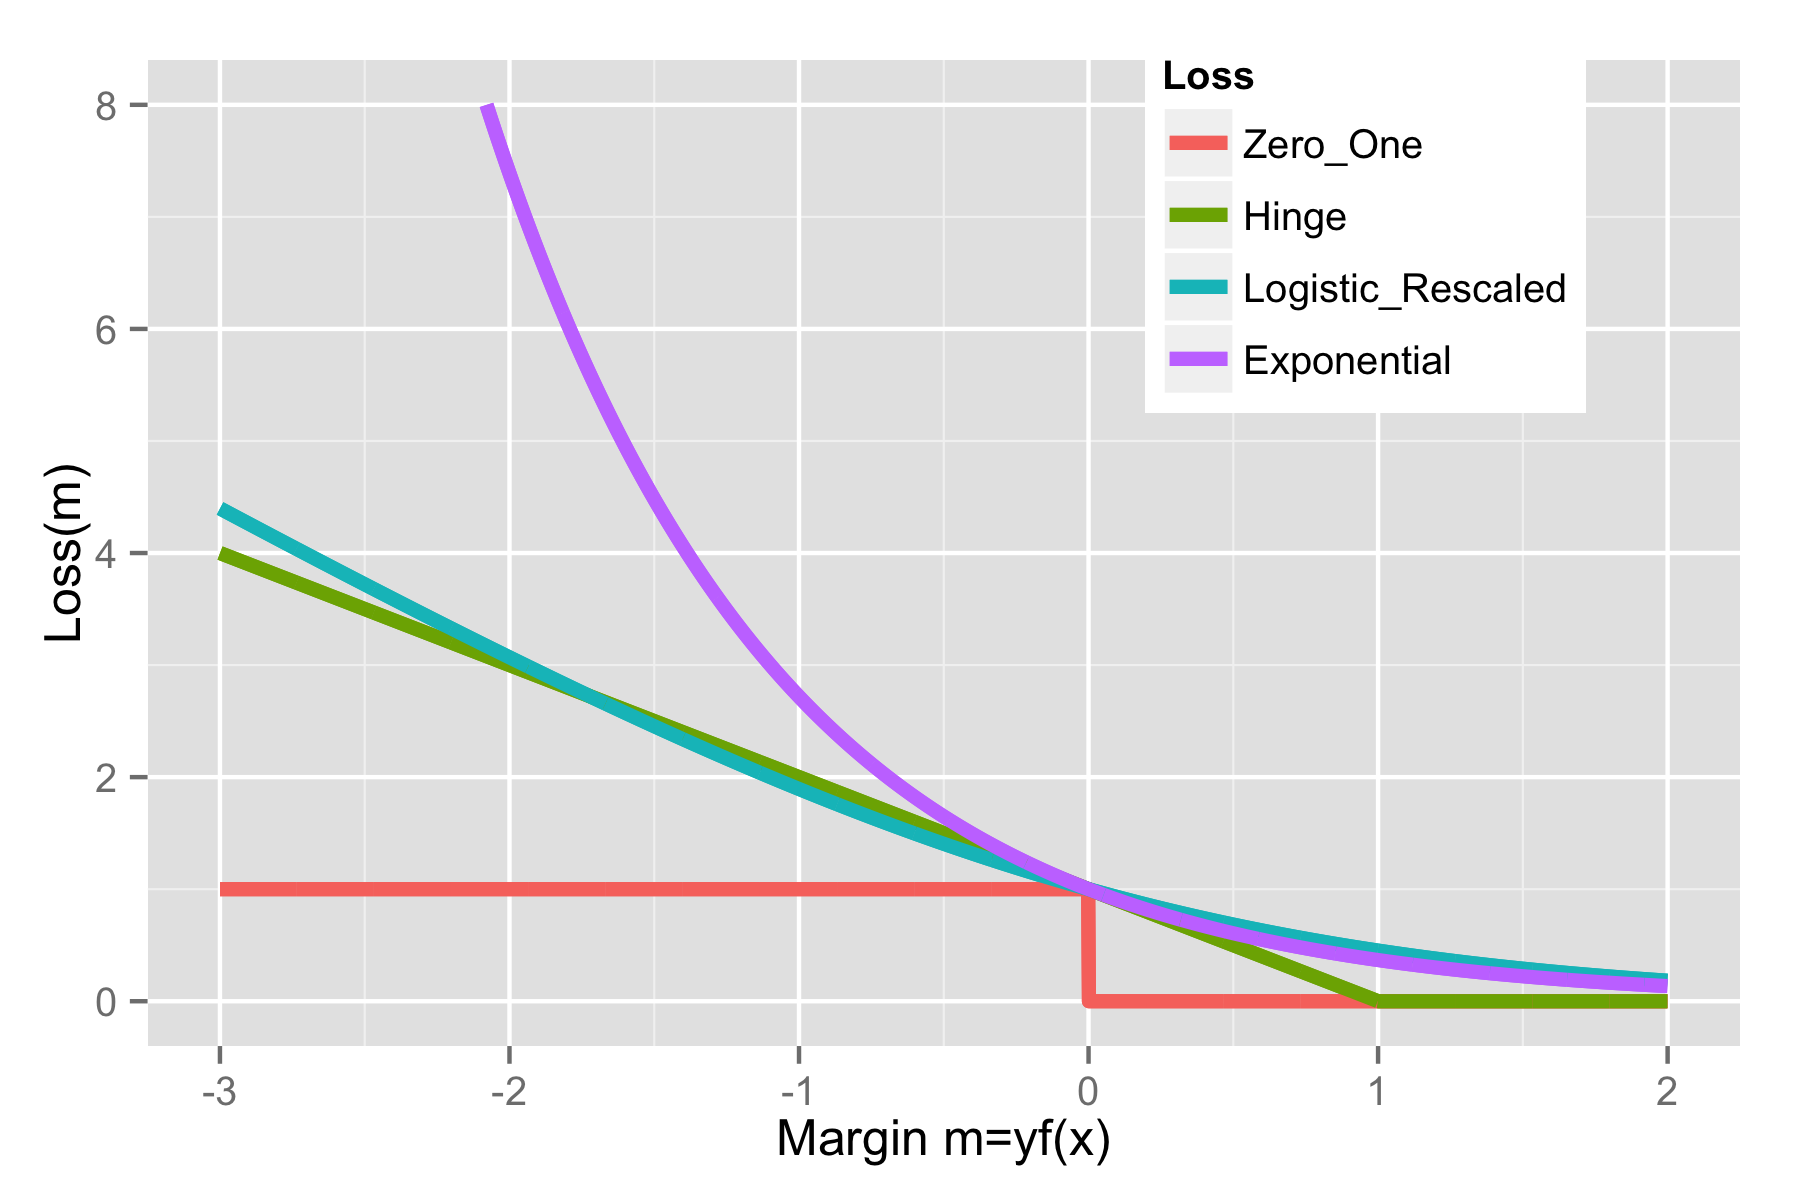
\includegraphics[height=0.65\textheight]{{figures/loss.Zero_One.Hinge.Logistic_Rescaled.Exponential}.png}
\par\end{center}
\note[item]{The exponential loss is just the exponential of negative margin. It is also a convex upperbound of the zero-one loss.}
\end{frame}
%
\begin{frame}{Forward Stagewise Additive Modeling with exponential loss}
Recall that we want to do FSAM with exponential loss.
\begin{enumerate}
\item Initialize $f_{0}(x)=0$.
\item For $m=1$ to $M$:
\begin{enumerate}
\item Compute:
\[
\left(v_{m},h_{m}\right)=\argmin_{v\in\reals,h\in\ch}\frac{1}{n}\sum_{i=1}^{n}{\color{blue}\ell_{\text{exp}}}\left(y_{i},f_{m-1}(x_{i})\underbrace{+v h(x_{i})}_{\text{new piece}}\right).
\]
\item Set $f_{m}=f_{m-1}+v_{m}h_m$.
\end{enumerate}
\item Return: $f_{M}$.
\end{enumerate}
\note[item]{Now let's plug in our loss function in FSAM.}
\end{frame}

\begin{frame}{FSAM with Exponential Loss: objective function}
\begin{itemize}
\item Base hypothesis: $\sH = \pc{h\colon \sX \rightarrow \pc{-1, 1}}$.
\item Objective function in the $m$'th round:
\pause
\begin{align}
J(v, h) &= \sum_{i=1}^n \exp\pb{
-y_i \p{ f_{m-1}(x_i) + vh(x_i) }
} \\
&= \sum_{i=1}^n w_i^m \exp\pb{ -y_ivh(x_i) } &&  \commenteq{w_i^m \eqdef \exp\pb{ -y_i f_{m-1}(x_i) } }\\
&= \sum_{i=1}^n w_i^m \pb{ \1\p{y_i=h(x_i)}e^{-v} + \1\p{y_i\neq h(x_i)}e^v } 
&& \commenteq{h(x_i) \in \pc{1, -1}} \\
&=  \sum_{i=1}^n w_i^m \pb{ (e^v-e^{-v})\1\p{y_i\neq h(x_i)} + e^{-v} }
&& \commenteq{\1\p{y_i=h(x_i)} = 1- \1\p{y_i\neq h(x_i)}}
\end{align}


\end{itemize}
\end{frame}
%
\begin{frame}{FSAM with Exponential Loss: basis function}
\begin{itemize}[<+->]
\item Objective function in the $m$'th round:
\begin{align}
J(v, h) &= \sum_{i=1}^n w_i^m \pb{ (e^v-e^{-v})\1\p{y_i\neq h(x_i)} + e^{-v} } .
\end{align}
\item If $v>0$, then
\begin{align}
\onslide<.->{
\argmin_{h\in\sH}J(v,h) &=
\argmin_{h\in\sH} \sum_{i=1}^n w_i^m \1\p{y_i\neq h(x_i)} \\
}
\onslide<+->{
h_m &= \argmin_{h\in\sH} \sum_{i=1}^n w_i^m \1\p{y_i\neq h(x_i)} \\
}
\onslide<+->{
&= \argmin_{h\in\sH} \frac{1}{\sum_{i=1}^n w_i^m} \sum_{i=1}^n w_i^m \1\p{y_i\neq h(x_i)}
&& \commenteq{\text{multiply by a positive constant}}
}
\end{align}
\onslide<+->{
\ie $h_m$ is the minimizer of the weighted zero-one loss.
}
\end{itemize}
\note[item]{Let's first find the optimal $h$, the last term does not depend on $h$ so it can be ignored for now. Do we want the indicator to be one or zero? It depends on the coefficient.}
\end{frame}

\begin{frame}{FSAM with Exponential Loss: classifier weights}
\begin{itemize}[<+->]
\item Define the weighted zero-one error:
\begin{align}
\text{err}_m = \frac{\sum_{i=1}^n w_i^m \1\p{y_i\neq h(x_i)}}{\sum_{i=1}^n w_i^m} .
\end{align}
\item \think{Exercise}: show that the optimal $v$ is:
\begin{align}
v_m = \frac{1}{2}\log\frac{1-\text{err}_m}{\text{err}_m}
\end{align}
\begin{itemize}
\item Same as the classifier weights in Adaboost (differ by a constant).
\item If $\text{err}_m < 0.5$ (better than chance), then $v_m > 0$.
\end{itemize}
\end{itemize}
\note[item]{Now let's fine the optimal weight $v$.}
\note[item]{To simplify notation, let's define $err_m$. Since $v$ is a real number, you can compute the gradient w.r.t. $v$ and set it to zero.}
\note[item]{Remember that we assumed $v>0$. Is it true for optimal $v$?}
\end{frame}

\begin{frame}
{FSAM with Exponential Loss: example weights}
\begin{itemize}
\item Weights in the next round:
\begin{align}
w_i^{m+1} &\eqdef \exp\pb{ -y_i f_m(x_i) } \\
\onslide<2->{
&= w_i^m \exp\pb{ -y_i v_m h_m(x_i) } 
\quad\quad\quad \commenteq{f_m(x_i) = f_{m-1}(x_i) + v_mh_m(x_i)} \\
&= w_i^m \exp\pb{ -v_m\1\p{y_i = h_m(x_i)} + v_m\1\p{y_i \neq h_m(x_i)} } \\
&= w_i^m \exp\pb{ 2v_m\1\p{y_i \neq h_m(x_i)} } \underbrace{\exp^{-v_m}}_{\text{scaler}}
}
\end{align}
\item<3-> The constant scaler will cancel out during normalization.
\item<4-> $2v_m = \alpha_m$ in Adaboost.
\end{itemize}
\note[item]{So far we have shown that FSAM with exponential loss also fits base classifiers using the weighted zero-one loss, and classifier weights is the same as Adaboost. But what about the example weights?}
\note[item]{The example weights are updated in the same way too! If an example is misclassified, we increase its weight same as in Adaboost.}
\note[item]{Now we have derived Adaboost using FSAM with exponential loss.}
\end{frame}

\begin{frame}{Why Exponential Loss}
\begin{itemize}[<+->]
\item $\ell_{\text{exp}}(y, f(x)) = \exp(-yf(x))$.
\item \think{Exercise}: show that the optimal estimate is
\begin{align}
f^*(x) = \frac{1}{2}\log\frac{p(y=1\mid x)}{p(y=0\mid x)} .
\end{align}
\item How is it different from other losses?
\begin{center}
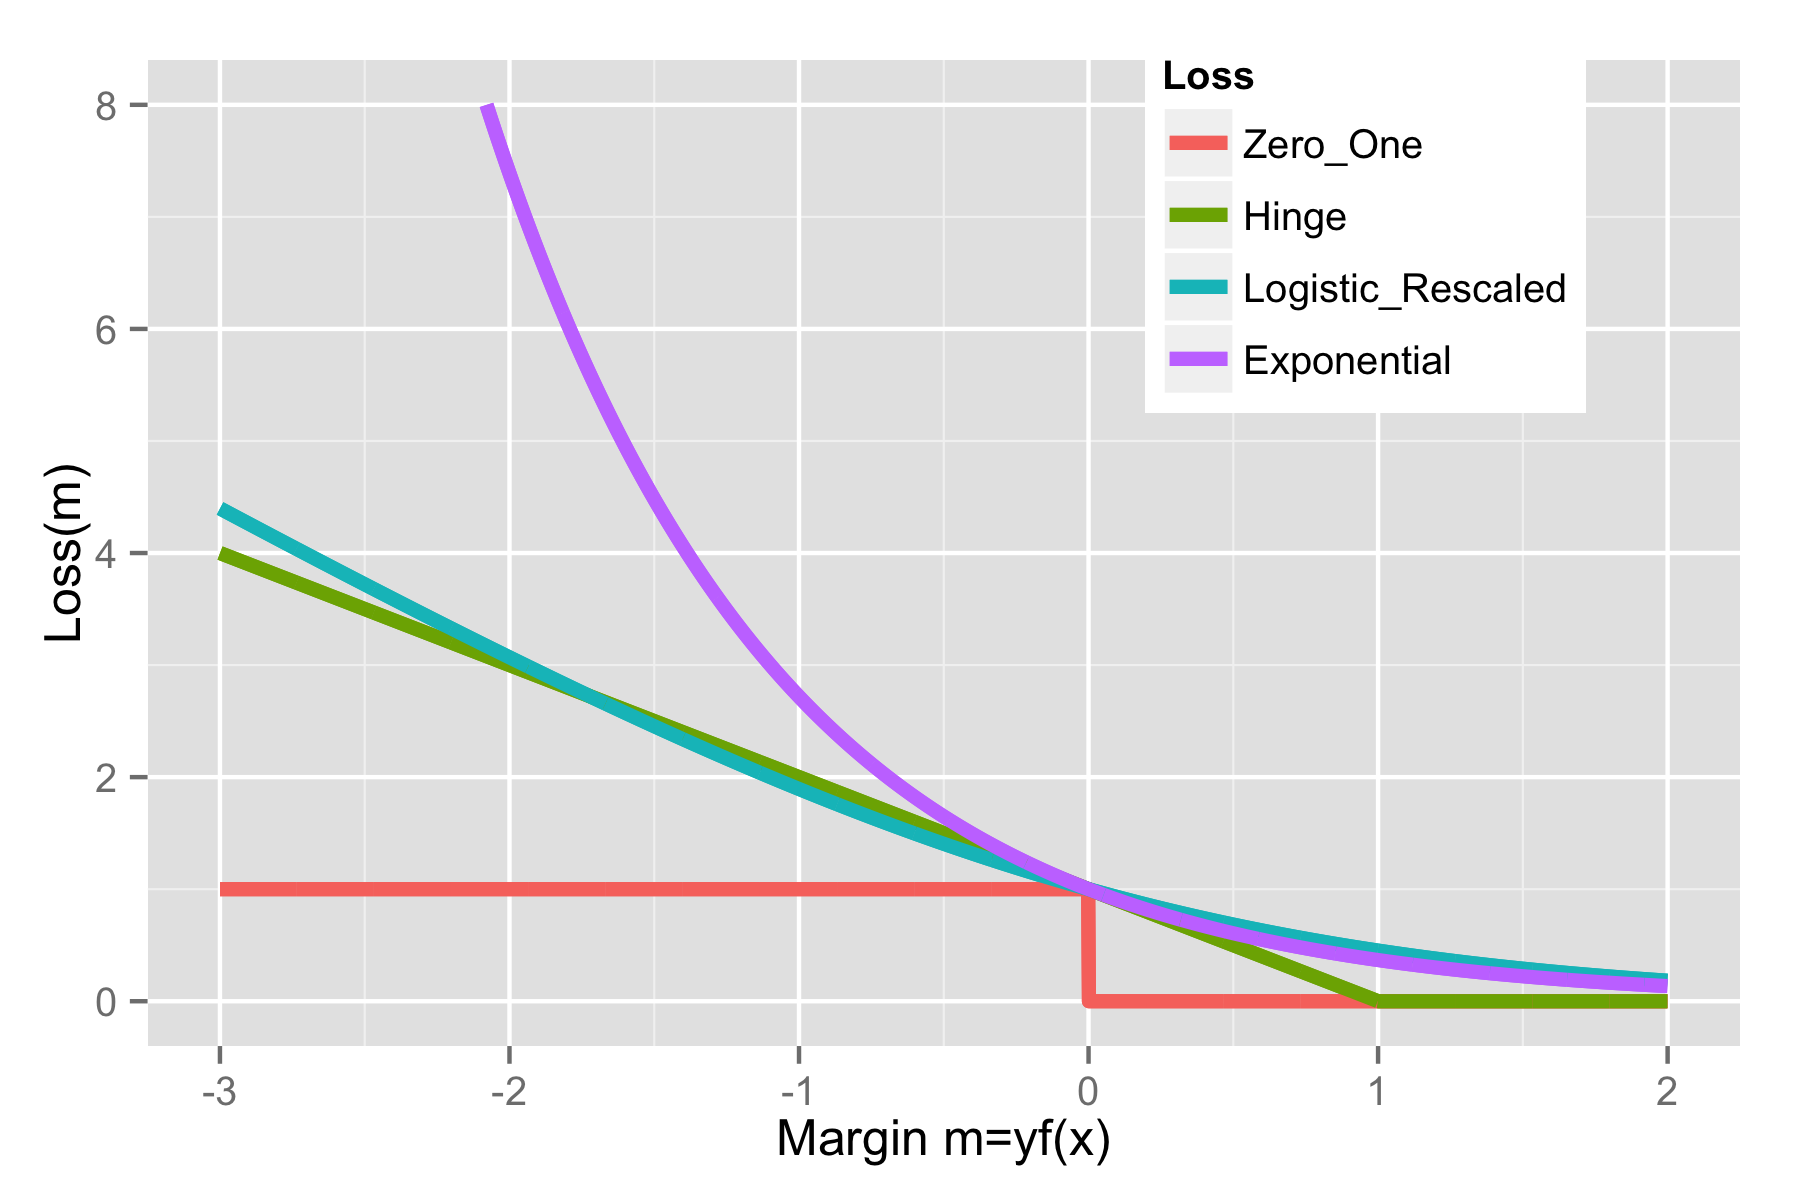
\includegraphics[height=0.45\textheight]{{figures/loss.Zero_One.Hinge.Logistic_Rescaled.Exponential}.png}
\end{center}
\end{itemize}
\note[item]{Adaboost was not initially designed to minimize exponential loss. It's only discovered 5 years after its invention. In the FSAM context, the main motivation for using exponential loss is computational: it leads to a simple optimization algorithm through example reweighting. But let's think about why this loss function makes sense from the statistical learning perspective.}
\note[item]{We can show that the optimal $f(x)$ is estimating one-half of the log odds. This justifies using the sign of it the make map the score to -1 and 1, \ie optimal under bayes decision rule.}
\note[item]{We have seen in logistic regression that its optimal estimate is also the log odds. So they will given the same model if there's infinite data. But in the finite-sample case, their behavior will be different.}
\note[item]{It puts more penalty on wrong predictions.}
\end{frame}
%
\begin{frame}{AdaBoost / Exponential Loss: Robustness Issues}
\begin{itemize}
\item Exponential loss puts a high penalty on misclassified examples.
\pause
\begin{itemize}
\item $\implies$ not robust to outliers / noise.
\end{itemize}
\item Empirically, AdaBoost has degraded performance in situations with 
\begin{itemize}
\item high Bayes error rate (intrinsic randomness in the label)
\end{itemize}
\pause
\item Logistic/Log loss performs better in settings with high Bayes error.
%\begin{itemize}
\item Exponential loss has some computational advantages over log loss though.
%\item FSAM + log loss $\implies$ LogitBoost
%\end{itemize}
\end{itemize}
\note[item]{Why is it bad? It means that the model will try very hard on a few misclassified examples.}
\end{frame}
%
\begin{frame}{Review}
We've seen
\begin{itemize}
\item Use basis function to obtain \emph{nonlinear} models: $f(x) = \sum_{i=1}^M v_m h_m(x)$ with known $h_m$'s.
\item \emph{Adaptive} basis function models: $f(x) = \sum_{i=1}^M v_m h_m(x)$ with unknown $h_m$'s.
\item Forward stagewise additive modeling: greedily fit $h_m$'s to minimize the average loss.
\end{itemize}
\pause
But,
\begin{itemize}
\item We only know how to do FSAM for certain loss functions.
\item Need to derive new algorithms for different loss functions.
\end{itemize}

Next, how to do FSAM in general.
\note[item]{Let's recap now. We started with the nonlinear regression problem. One way to obtain nonlinear classifier in the linear form is through basis functions, which compute a nonlinear transformation of $x$.}
\note[item]{If $h_m$ is known, that's easy---the problem is reduced to linear models. But what if we want to learn $h_m$'s?}
\note[item]{Last week we saw how to use the iterative Adaboost algorithm to find these base classifiers or basis functions. Today we saw that it's a special case of FSAM using exponential loss.}
\note[item]{In the FSAM framework, it is easy to plug in new loss functions.}
\end{frame}
%

\section{Gradient Boosting / ``Anyboost''}
\subsection{Motivating example: L2 Boosting}
\begin{frame}{FSAM with squared loss}
\begin{itemize}[<+->]
\item Objective function at $m$'th round:
\[
J(v,h)=\frac{1}{n}\sum_{i=1}^{n}\left(y_{i}-\left[f_{m-1}(x_{i})\underbrace{+v h(x_{i})}_{\text{new piece}}\right]\right)^{2}
\]

\item If $\ch$ is closed under rescaling (i.e. if $h\in\ch$, then $vh\in\ch$
for all $h\in\reals$), then don't need $v$.

\item Take $v=1$ and minimize
\[
J(h)=\frac{1}{n}\sum_{i=1}^{n}\left(\left[\underbrace{y_{i}-f_{m-1}(x_{i})}_{\onslide<+->{\text{residual}}}\right]-h(x_{i})\right)^{2}
\]

\item This is just fitting the residuals with least-squares regression!
\item<.-> Example base hypothesis space: regression stumps.
\end{itemize}
\note[item]{Let's consider FSAM with squared loss a s a motivating example.}
\note[item]{Remember that in each round of FSAM we minimize the empirical risk, which is the average loss on the training data. And we only fit one basis function without changing the previous ones.}
\note[item]{Now, we want to find $h$ in our base hypothesis space that minimizes $J$. First notice that if $\sH$ is closed under rescaling, meaning that if a function is in $\sH$ then its scaled version also belongs to $\sH$. Then we can consider $vh$ as another function $g$. Basically we can ignore $v$ if we assume...}
\note[item]{Now, let's re-arrange the terms. How do we interpret the first term?}
\note[item]{It's the residuals, so minimizing $J$ is equivalent to fit the residuals with squared loss.}
\end{frame}
%
%\begin{frame}{Regression Stumps}
%\begin{itemize}
%\item A \textbf{regression stump }is a regression tree with a single split.
%\item A\textbf{ regression stump }is a function of the form \textbf{$h(x)=a\ind{x_{i}\le c}+b\ind{x_{i}>c}$.}
%\end{itemize}
%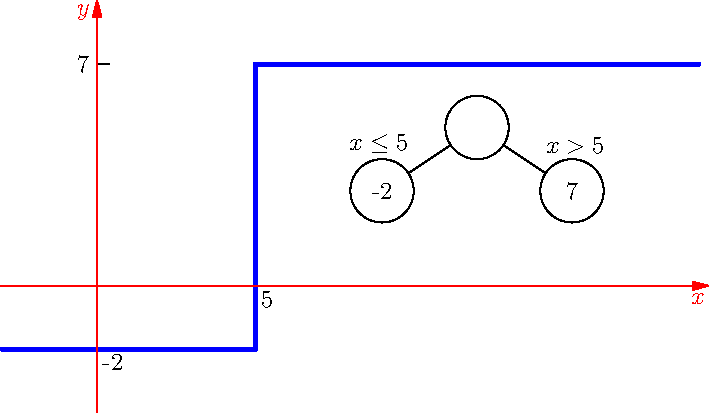
\includegraphics[clip,height=0.7\textheight]{figures/stump}
%\let\thefootnote\relax\footnotetext{\tiny{Plot courtesy of Brett Bernstein.}}
%\end{frame}
%%
\begin{frame}{$L^{2}$ Boosting with Decision Stumps: Demo}
\begin{itemize}
\item Consider FSAM with $L^{2}$ loss (i.e. $L^{2}$ Boosting)
\item For base hypothesis space of \textbf{regression stumps}
\end{itemize}

%\begin{itemize}
%\item Data we'll fit with \href{https://davidrosenberg.github.io/mlcourse/Labs/gbm.py}{code}:
%\end{itemize}
\begin{figure}
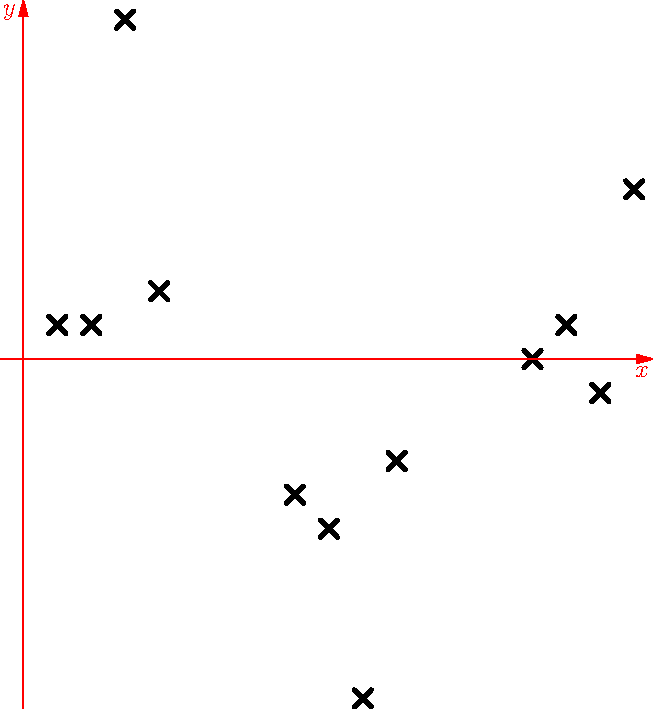
\includegraphics[clip,height=0.6\textheight]{figures/data}
\end{figure}

\let\thefootnote\relax\footnotetext{\tiny{Plot courtesy of Brett Bernstein.}}
\note[item]{Let's look at an example now to go over each round of FSAM with squared loss, which is also called L2 boosting. Our base hypothesis space is regression stumps, which is a regression tree with one split.}
\note[item]{Here's our data. Obviously it's non-linear.}
\end{frame}
%
\begin{frame}{$L^{2}$ Boosting with Decision Stumps: Results}
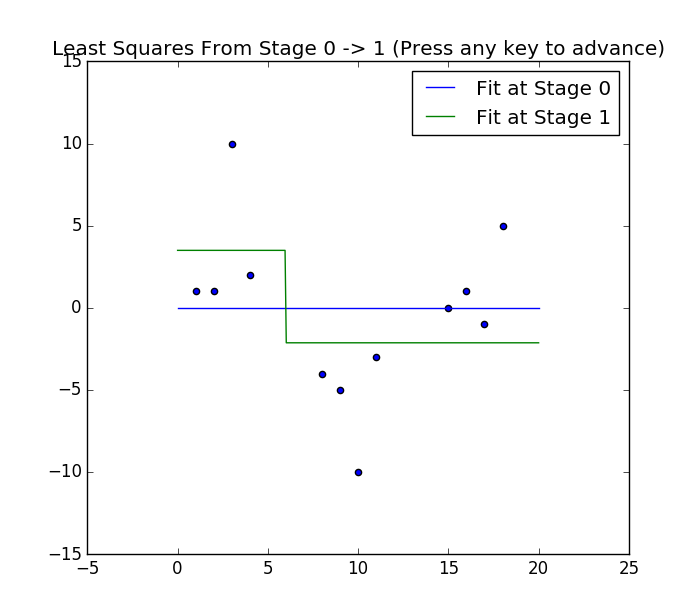
\includegraphics[height=0.8\textheight]{figures/l2boosting-stage1}%
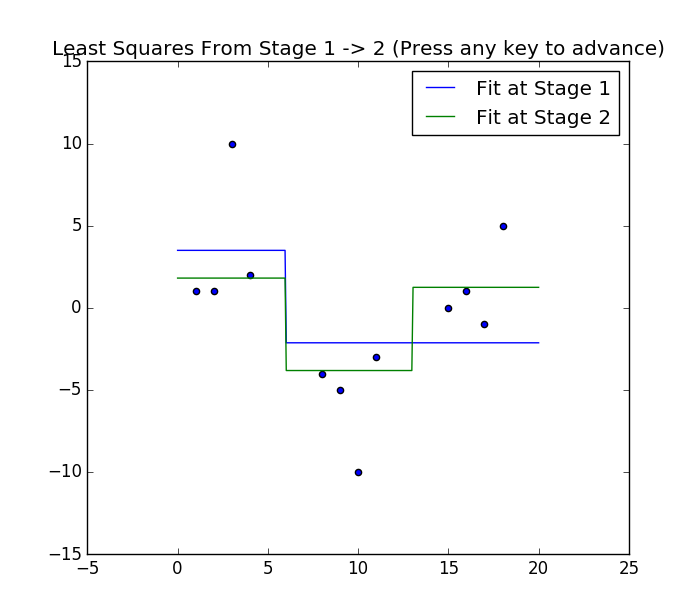
\includegraphics[height=0.8\textheight]{figures/l2boosting-stage2}
\let\thefootnote\relax\footnotetext{\tiny{Plots and code courtesy of Brett Bernstein.}}
\note[item]{Initially, our predictor is constant 0.}
\note[item]{Our first regression stump is the green line.}
\note[item]{In the next stage, we start with the sum of previous predictors, which is the blue line in the right figure.}
\note[item]{We add another decision stump which gives us the green line.}
\end{frame}
%
\begin{frame}{$L^{2}$ Boosting with Decision Stumps: Results}
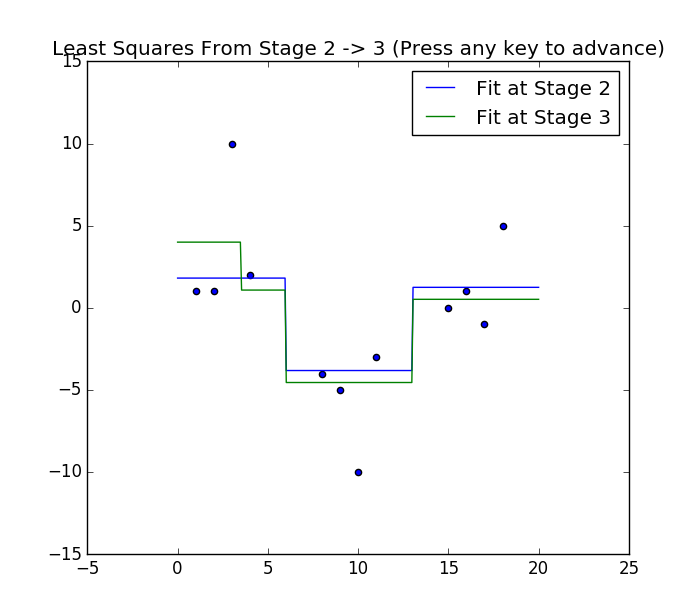
\includegraphics[height=0.8\textheight]{figures/l2boosting-stage3}%
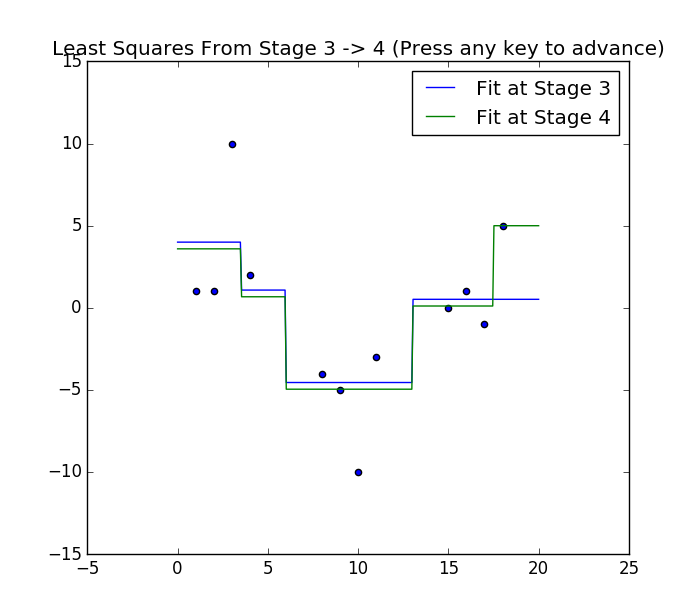
\includegraphics[height=0.8\textheight]{figures/l2boosting-stage4}
\let\thefootnote\relax\footnotetext{\tiny{Plots and code courtesy of Brett Bernstein.}}
\note[item]{So each time we add a new decision stump, so on and so forth.}
\end{frame}
%
\begin{frame}{$L^{2}$ Boosting with Decision Stumps: Results}

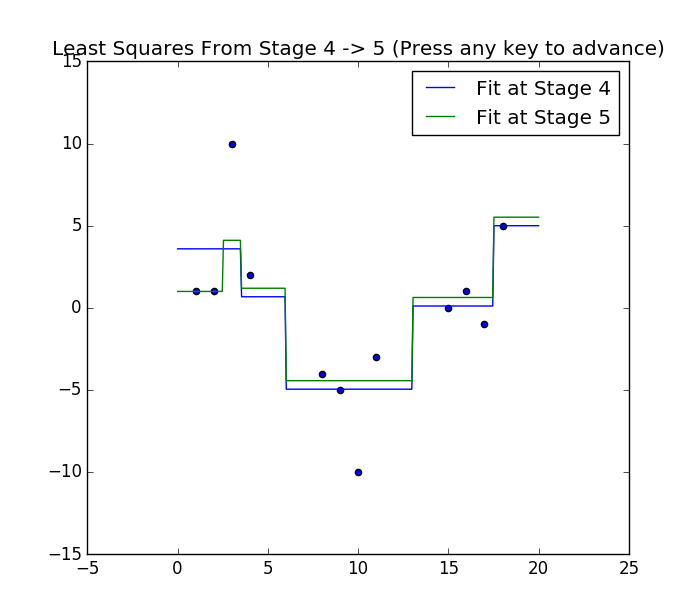
\includegraphics[height=0.8\textheight]{figures/l2boosting-stage5}%
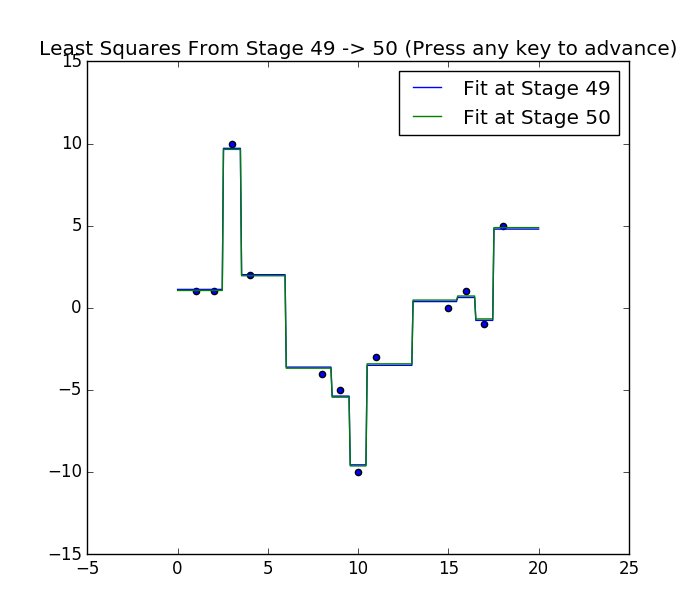
\includegraphics[height=0.8\textheight]{figures/l2boosting-stage50}
\let\thefootnote\relax\footnotetext{\tiny{Plots and code courtesy of Brett Bernstein.}}
\note[item]{After 50 stages, we can see that it overfitted. We will talk about how to prevent overfitting at the end.}
\note[item]{To summarize, in each round, we make a local improvement of our loss function. Specifically, here we move towards the target value incrementally. Now this process is actually quite similar to gradient descent, where we move along the direction that locally minimizes the objective. Next, let's consider its connection to gradient descent in a more formal way.}
\end{frame}

\begin{frame}
{Interpret the residual}
\begin{itemize}[<+->]
\item Objective: $J(f) = \frac{1}{n}\sum_{i=1}^n \p{y_i - f(x_i)}^2 $.
\item What is the residual at $x=x_i$?
\begin{align}
\frac{\partial}{\partial f(x_i)} J(f) = \onslide<+->{ -2 \p{y_i - f(x_i)} }
\end{align}
\begin{itemize}[<.->]
\item Gradient w.r.t. $f$: how should the output of $f$ change to minimize the squared loss.
\item \emph{Residual is the negative gradient} (differ by some constant).
\end{itemize}
\item At each boosting round, we learn a function $h\in\sH$ to fit the residual.
\begin{align}
f &\leftarrow f + {\color{red}v}{\color{Green}h} && \text{FSAM / boosting} \\
\onslide<+->{
f &\leftarrow f - {\color{red}\alpha}{\color{Green}\nabla_f J(f)} && \text{gradient descent}
}
\end{align}
\begin{itemize}[<.->]
\item $h$ approximates the gradient (step direction).
\item $v$ is the step size.
\end{itemize}
\end{itemize}
\note[item]{So this is our loss function. Let's consider the value of $f$ at each training point $x_i$ as a variable that we can optimize.}
\note[item]{Then we can take gradient w.r.t. $f(x_i)$. That means how should we change the output at $x_i$ to minimize $J$.}
\note[item]{In FSAM, in each round we add a weighted basis function.}
\note[item]{Let's compare that with gradient descent. If we consider $f$ as a vector, then in each step, we move the vector along the negative gradient at the current value of $f$.}
\end{frame}

\subsection{Gradient Descent in the Function Space}

%\begin{frame}{FSAM Is Iterative Optimization}
%\begin{itemize}
%\item The FSAM step
%\[
%\left(v_{m},h_{m}\right)=\argmin_{v\in\reals,h\in\ch}\sum_{i=1}^{n}\ell\left(y_{i},f_{m-1}(x_{i})\underbrace{+v h(x_{i})}_{\text{new piece}}\right).
%\]
%
%
%\pause{}
%\item Hard part: finding the \textbf{best} \textbf{step direction} $h$.
%
%\pause{}
%\item What if we looked for the \textbf{locally best }step direction?
%\begin{itemize}
%\item like in gradient descent
%\end{itemize}
%\end{itemize}
%\end{frame}
%%
\begin{frame}{``Functional'' Gradient Descent }
\begin{itemize}
\item We want to minimize
\[
J(f)=\sum_{i=1}^{n}\ell\left(y_{i},f(x_{i})\right).
\]
\item In some sense, we want to take the gradient w.r.t. $f$.

\pause{}
\item $J(f)$ only depends on $f$ at the $n$ training points.

\pause{}
\item Define ``parameters''
\[
{\bf f}=\left(f(x_{1}),\ldots,f(x_{n})\right)^{T}
\]
and write the objective function as 
\[
J({\bf f})=\sum_{i=1}^{n}\ell\left(y_{i,}{\bf f}_{i}\right).
\]
\end{itemize}
\note[item]{We want to minimize $J$ w.r.t. the function $f$ by gradient descent, so the hard part is to compute the gradient, or the step direction.}
\note[item]{Notice that the objective only depends on the value of $f$ at $n$ points and doesn't really care about values elsewhere.}
\note[item]{So let's reformulate the problem by vectorizing $f$ into an $n$-dim vector. Now it becomes a familiar problem---we can easily take gradient w.r.t. this vector $f$.}
\end{frame}
%
\begin{frame}{Functional Gradient Descent: Unconstrained Step Direction}
\begin{itemize}[<+->]
\item Consider gradient descent on 
\[
J({\mathbf{f}})=\sum_{i=1}^{n}\ell\left(y_{i,}{\bf f}_{i}\right).
\]

\item The {negative gradient step direction} at ${\bf f}$ is
\begin{eqnarray*}
-{\bf g} & = & -\del_{\vf}J({\bf f})\\
 & = & -\left(\partial_{{\bf f}_{1}}\ell\left(y_{1},{\bf f}_{1}\right),\ldots,\partial_{{\bf f}_{n}}\ell\left(y_{n},{\bf f}_{n}\right)\right)
\end{eqnarray*}
which we can easily calculate.

\item<.-> $-{\bg}\in\reals^{n}$ is the direction we want to change each of
our $n$ predictions on training data.

\item With gradient descent, our final predictor will be an additive model: $f_0+\sum_{m=1}^M v_t (-\bg_t)$.
\end{itemize}

\note[item]{So what is our gradient now?}
\note[item]{The gradient is simply the vector of partial derivatives w.r.t. $f_i$'s. So now we have the direction towards which we can move our function $f$ at each training points.}
\note[item]{Starting with $f_0=0$, we will get an additive model with gradient descent.}
\end{frame}
%
\begin{frame}{Functional Gradient Descent: Projection Step}
\begin{itemize}[<+->]
\item Unconstrained step direction is
\[
-{\bg}=-\del_{\vf}J({\bf f})=-\left(\partial_{{\bf f}_{1}}\ell\left(y_{1},{\bf f}_{1}\right),\ldots,\partial_{{\bf f}_{n}}\ell\left(y_{n},{\bf f}_{n}\right)\right).
\]
\begin{itemize}[<.->]
\item Also called the ``\textbf{pseudo-residuals}''.
(For squared loss, they're exactly the residuals.)
\end{itemize}

\item 
\alarm{Problem}: only know how to update $\bf$ at $n$ points. How do we take a  gradient step in $\sH$?
\item \emph{Solution}: approximate by the closest base hypothesis $h\in\ch$ (in the $\ell^{2}$ sense):
\begin{align}
\min_{h\in\ch}\sum_{i=1}^{n}\left(-{\bf g}_{i}-h(x_{i})\right)^{2}.
&& \text{least square regression}
\end{align}

\item<.-> Take the $h\in\ch$ that best approximates $-{\bf g}$ as our step
direction.
\end{itemize}
\note[item]{However, our gradient is only defined on $n$ points. In other words, it is in $\reals^n$. But we want an update in the base hypothesis space. In other words, we want to project $g$ to $\sH$.}
\note[item]{So the problem now becomes finding a function in $\sH$ whose values at $x_i$'s are closest to the gradient vector, which is basically a regression problem.}
\end{frame}



\begin{frame}
{Recap}
\begin{itemize}[<+->]
\item Objective function: 
\begin{align}
J(f) = \sum_{i=1}^n \ell(y_i, f(x_i)) .
\end{align}
\item Unconstrained gradient $\bg \in \reals^n$ w.r.t. ${\vf}=(f(x_1), \ldots, f(x_n))^T$:
\begin{align}
{\bg}=\del_{\vf}J({\bf f})=\left(\partial_{{\bf f}_{1}}\ell\left(y_{1},{\bf f}_{1}\right),\ldots,\partial_{{\bf f}_{n}}\ell\left(y_{n},{\bf f}_{n}\right)\right).
\end{align}
\item Projected negative gradient $h \in \sH$:
\begin{align}
h = \argmin_{h\in\ch}\sum_{i=1}^{n}\left(-{\bf g}_{i}-h(x_{i})\right)^{2}.
\end{align}
\item Gradient descent:
\begin{align}
f \leftarrow f + {\color{red}v}h
\end{align}
\end{itemize}
\note[item]{But we still need to figure out the step size $v$.}
\end{frame}

\begin{frame}{Functional Gradient Descent: hyperparameters}
\begin{itemize}
\item Choose a step size by \textbf{line search}. 
\[
v_{m}=\argmin_{v}\sum_{i=1}^{n}\ell\left\{ y_{i},f_{m-1}(x_{i})+v h_{m}(x_{i})\right\} .
\]
\begin{itemize}
\item Not necessary. Can also choose a fixed hyperparameter $v$.
\end{itemize}
\item Regularization through \textbf{shrinkage}:
\begin{align}
f_m \leftarrow f_{m-1} + {\color{blue}\lambda} v_m h_m \quad \text{where}\; \lambda \in \pb{0,1} .
\end{align}
\begin{itemize}
\item Typically choose $\lambda = 0.1 $.
\end{itemize}

\item Choose $M$, \ie when to stop.
\begin{itemize}
\item Tune on validation set.
\end{itemize}
\end{itemize}
\note[item]{Now that we know $h_m$, we can solve another optimization problem to find the best $v_m$ that minimizes the objective.}
\note[item]{An alternative is to fix the step size, which can be tuned on the validation set.}
\end{frame}
%
\begin{frame}
{Gradient boosting algorithm}
\begin{enumerate}
\item Initialize $f$ to a constant: $f_0(x) = \argmin_\gamma \sum_{i=1}^n \ell(y_i, \gamma)$.
\item For $m$ from $1$ to $M$:
\begin{enumerate}
\item Compute the pseudo-residuals (negative gradient):
\begin{align}
r_{im} = -\pb{ \frac{\partial}{\partial f(x_i)} \ell(y_i, f(x_i) }_{f(x_i) = f_{m-1}(x_i)}
\end{align}
\item Fit a base learner $h_m$ with squared loss using the dataset $\pc{(x_i, r_{im})}_{i=1}^n$.
\item {[Optional]} Find the best step size $v_m = \argmin_v \sum_{i=1}^n \ell\p{yi, f_{m-1}(x_i) + vh_m(x_i)}.$
\item Update $f_m = f_{m-1} + \lambda v_mh_m$
\end{enumerate}
\item Return $f_M(x)$.
\end{enumerate}
\end{frame}

\begin{frame}{The Gradient Boosting Machine Ingredients (Recap)}
\begin{itemize}
\item Take any loss function {[}sub{]}differentiable w.r.t. the prediction $f(x_i)$
\item Choose a base hypothesis space for regression.
\item Choose number of steps (or a stopping criterion).
\item Choose step size methodology.
\item Then you're good to go!
\end{itemize}
\end{frame}
%

\subsection{Example: BinomialBoost}
\begin{frame}{BinomialBoost: Gradient Boosting with Logistic Loss}
\begin{itemize}
\item Recall the logistic loss for classification, with $\cy=\left\{ -1,1\right\} $:
\begin{eqnarray*}
\ell(y,f(x)) & = & \log\left(1+e^{-yf(x)}\right)
\end{eqnarray*}
\end{itemize}

\pause{}
\begin{itemize}
\item Pseudoresidual for $i$'th example is negative derivative of loss
w.r.t. prediction:
\begin{align}
r_{i} &= -\frac{\partial}{\partial f(x_i)} \ell(y_i, f(x_i)) \\ 
 &= -\frac{\partial}{\partial f(x_i)} \left[\log\left(1+e^{-y_{i}f(x_{i})}\right)\right]\\
 &= \frac{y_{i}e^{-y_{i}f(x_{i})}}{1+e^{-y_{i}f(x_{i})}}\\
 &= \frac{y_{i}}{1+e^{y_{i}f(x_{i})}}
\end{align}
\end{itemize}
\end{frame}
%
\begin{frame}{BinomialBoost: Gradient Boosting with Logistic Loss}
\begin{itemize}
\item Pseudoresidual for $i$th example:
\begin{eqnarray*}
r_{i} & = & -\frac{\partial}{\partial f(x_i)}\left[\log\left(1+e^{-y_{i}f(x_{i})}\right)\right]=\frac{y_{i}}{1+e^{y_{i}f(x_{i})}}
\end{eqnarray*}
\end{itemize}

\pause{}
\begin{itemize}
\item So if $f_{m-1}(x)$ is prediction after $m-1$ rounds, step direction
for $m$'th round is
\end{itemize}
\[
h_{m}=\argmin_{h\in\ch}\sum_{i=1}^{n}\left[\left(\frac{y_{i}}{1+e^{y_{i}f_{m-1}(x_{i})}}\right)-h(x_{i})\right]^{2}.
\]


\pause{}
\begin{itemize}
\item And $f_{m}(x)=f_{m-1}(x)+v h_{m}(x).$
\end{itemize}
\note[item]{This pseudo residuals are our targets of the function at $n$ points. So what's our regression problem?}
\end{frame}

\subsection{Gradient Tree Boosting}
\begin{frame}{Gradient Tree Boosting}
\begin{itemize}
\item One common form of gradient boosting machine takes
\[
\ch=\left\{ \mbox{regression trees of size \ensuremath{S}}\right\} ,
\]
where $S$ is the number of terminal nodes.

\item $S=2$ gives decision stumps

\item HTF recommends $4\le S\le8$ (but more recent results use much larger
trees)
\item Software packages:
\begin{itemize}
\item Gradient tree boosting is implemented by the {gbm package}
for R
\item as \texttt{\footnotesize{}GradientBoostingClassifier} and \texttt{\footnotesize{}GradientBoostingRegressor}
in {sklearn}
\item {xgboost} and {lightGBM} are state of the art for speed
and performance
\end{itemize}
\end{itemize}
\end{frame}

\begin{frame}{Sinc Function: Our Dataset}

\begin{figure}
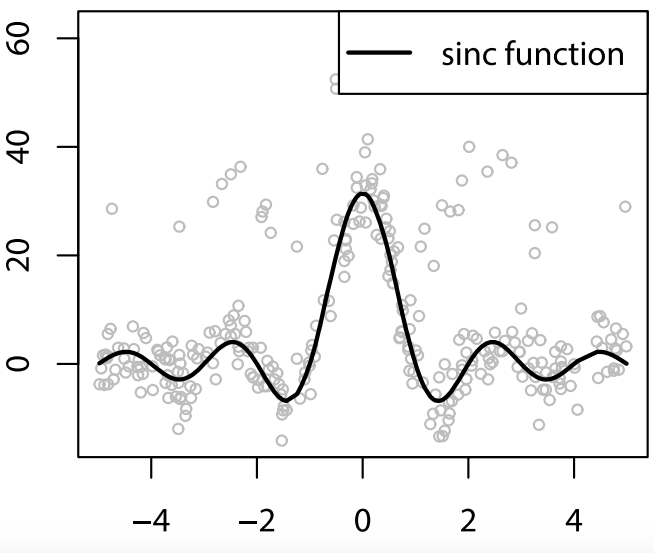
\includegraphics[height=0.6\textheight]{figures/sinc-fn-data}
\end{figure}

\let\thefootnote\relax\footnotetext{\tiny{From Natekin and Knoll's "Gradient boosting machines, a tutorial"}}
\end{frame}
%
\begin{frame}{Minimizing Square Loss with Ensemble of Decision Stumps}
\begin{center}
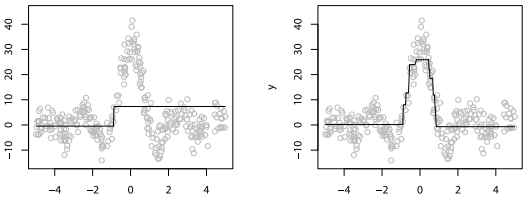
\includegraphics[height=0.3\textheight]{figures/sinc-fit-1step10steps}

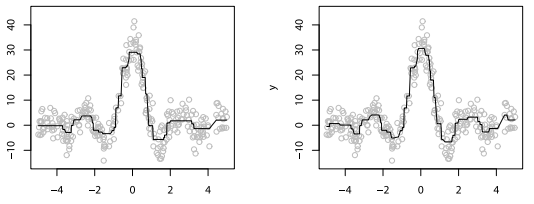
\includegraphics[height=0.3\textheight]{figures/sinc-fit-50steps100steps} 
\end{center}
Decision stumps with $1,10,50$, and $100$ steps, shrinkage $\lambda=1$.

\let\thefootnote\relax\footnotetext{\tiny{Figure 3 from Natekin and Knoll's "Gradient boosting machines, a tutorial"}}

\note[item]{A simple step function can be boosted to fit nonlinear data.}
\end{frame}
%

\section{Gradient Boosting in Practice}
\begin{frame}
{Prevent overfitting}
\begin{itemize}
\item Boosting is resistant to overfitting. Some explanations:
\begin{itemize}
\item Implicit feature selection: greedily selects the best feature (weak learner)
\item As training goes on, impact of change is localized.
\end{itemize}

\item But it can of course overfit. Common regularization methods:
\begin{itemize}
\item Shrinkage (small learning rate)
\item Stochastic gradient boosting (row subsampling)
\item Feature subsampling (column subsampling)
\end{itemize}
\end{itemize}
\end{frame}

\begin{frame}{Step Size as Regularization}

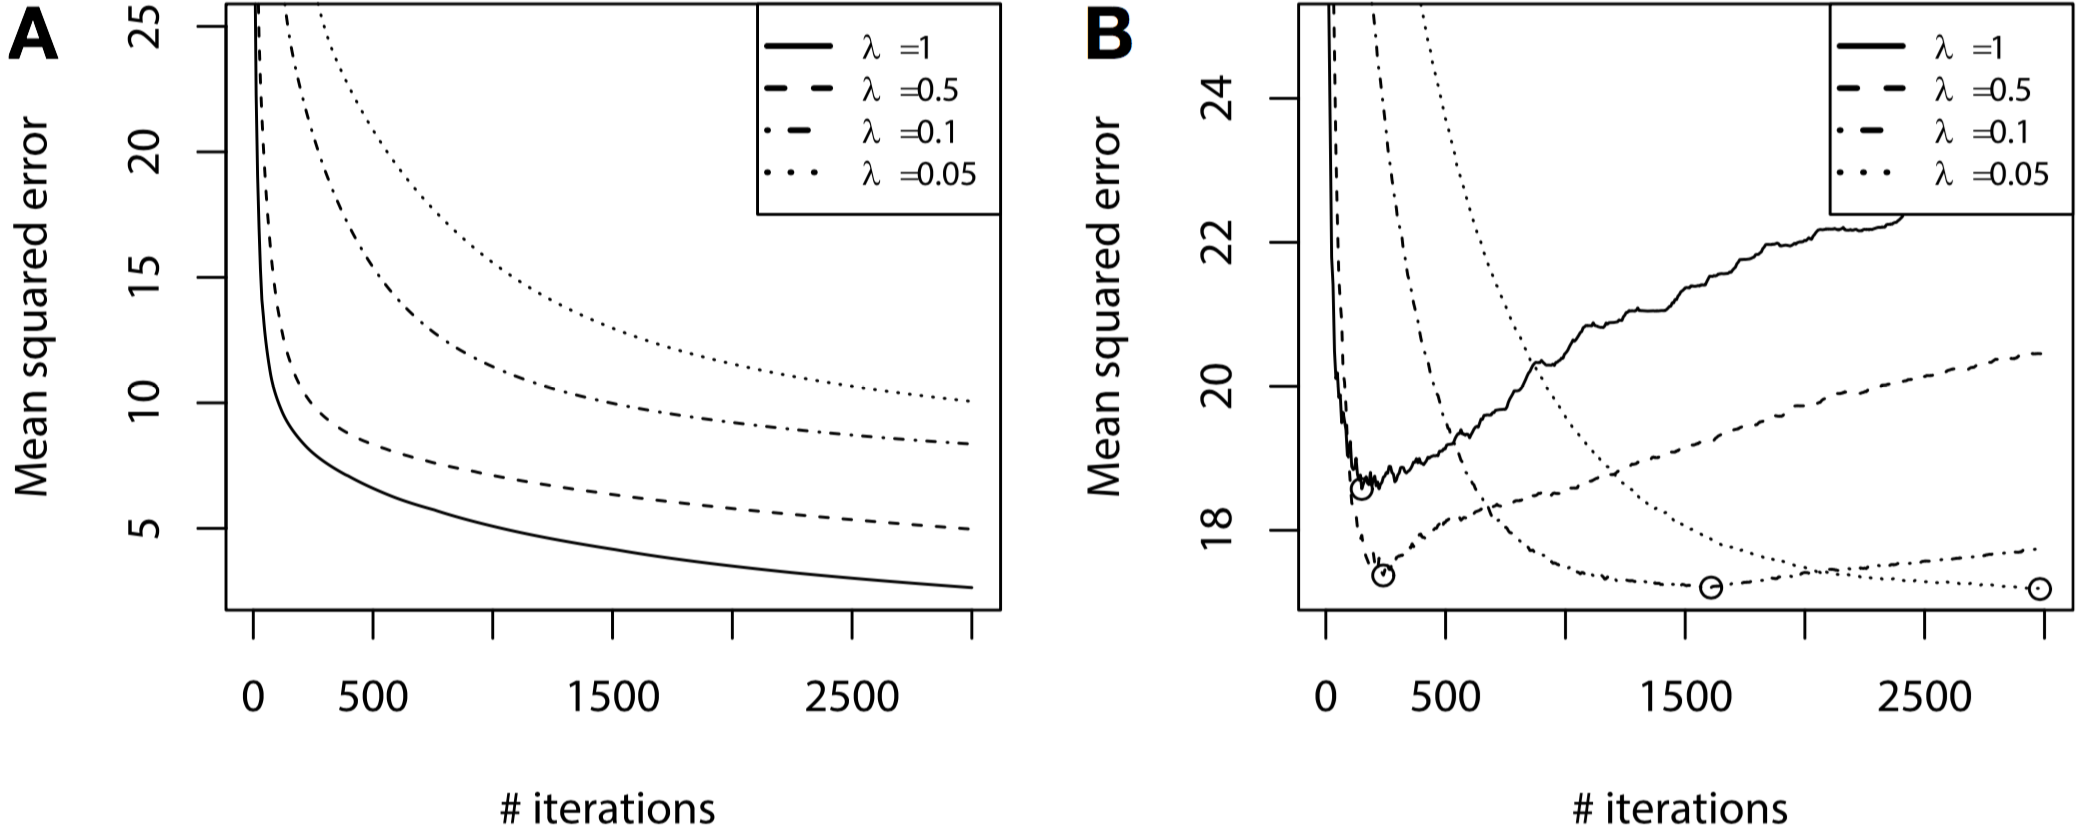
\includegraphics[width=0.8\textwidth]{figures/sinc-regression-train-validation} 

\begin{itemize}
\item (continued) sinc function regression
\item Performance vs rounds of boosting and shrinkage. (Left is training
set, right is validation set)
\end{itemize}

\let\thefootnote\relax\footnotetext{\tiny{Figure 5 from Natekin and Knoll's "Gradient boosting machines, a tutorial"}}
\note[item]{Left is training: larger step size leads to lower training loss as it updates more aggressively.}
\note[item]{Right is validation: larger step size converges faster but also converge to a worse solution.}
\end{frame}
%
\begin{frame}{Rule of Thumb}
\begin{itemize}
\item The smaller the step size, the more steps you'll need.
\item But never seems to make results worse, and often better.
\item So set your step size as small as you have patience for.
\end{itemize}
\note[item]{Next let's consider subsampling method.}
\end{frame}

\begin{frame}{Stochastic Gradient Boosting}
\begin{itemize}[<+->]
\item For each stage, 
\begin{itemize}[<.->]
\item choose random \emph{subset of data} for computing projected gradient step.
\end{itemize}
\item Why do this?
\begin{itemize}[<.->]
\item Introduce randomization thus may help overfitting.
\item Faster; often better than gradient descent given the same computation resource.
\end{itemize}
\item We can view this is a \textbf{minibatch method}. 
\begin{itemize}[<.->]
\item Estimate the ``true'' step direction
using a subset of data.
\end{itemize}
\let\thefootnote\relax\footnotetext{\tiny{Introduced by Friedman (1999) in \href{http://statweb.stanford.edu/~jhf/ftp/stobst.pdf}{Stochastic Gradient Boosting}. }}
\end{itemize}
\end{frame}
%
%\begin{frame}{Bag as Minibatch}
%\begin{itemize}
%\item Just as we argued for minibatch SGD, 
%\begin{itemize}
%\item sample size needed for a good estimate of step direction is independent
%of training set size
%\end{itemize}
%
%\pause{}
%\item Minibatch size should depend on 
%\begin{itemize}
%\item the complexity of base hypothesis space
%\item the complexity of the target function (Bayes decision function)
%\end{itemize}
%
%\pause{}
%\item Seems like an interesting area for both practical and theoretical
%pursuit.
%\end{itemize}
%\end{frame}
%

\begin{frame}{Column / Feature Subsampling}
\begin{itemize}
\item Similar to random forest, randomly choose \emph{a subset of features} for
each round.

\item XGBoost paper says: ``According to user feedback, using column sub-sampling
prevents overfitting even more so than the traditional row sub-sampling.''

\item Speeds up computation.
\end{itemize}
\end{frame}

%\begin{frame}{Newton Step Direction}
%\begin{itemize}
%\item For GBM, we find the closest $h\in\cf$ to the negative gradient
%\[
%-{\bf g}=-\del_{\vf}J({\bf f}).
%\]
%\item This is a ``first order'' method. 
%\end{itemize}
%
%\pause{}
%\begin{itemize}
%\item Newton's method is a ``second order method'':
%\begin{itemize}
%\item Find 2nd order (quadratic) approximation to $J$ at $\vf$.
%\begin{itemize}
%\item Requires computing gradient and Hessian of $J$.
%\end{itemize}
%\item Newton step direction points towards minimizer of the quadratic.
%\item Minimizer of quadratic is easy to find in closed form
%\end{itemize}
%
%\pause{}
%\item Boosting methods with projected Newton step direction:
%\begin{itemize}
%\item LogitBoost (logistic loss function)
%\item XGBoost (any loss \textendash{} uses regression trees for base classifier)
%\end{itemize}
%\end{itemize}
%\end{frame}
%%
%\begin{frame}{Newton Step Direction for GBM}
%\begin{itemize}
%\item Generically, second order Taylor expansion of $J$ at ${\bf f}$ in
%direction ${\bf r}$
%\[
%J({\bf f}+{\bf r})=J({\bf f})+\left[\del_{{\bf f}}J({\bf f})\right]^{T}{\bf r}+\frac{1}{2}{\bf r}^{T}\left[\del_{{\bf f}}^{2}J({\bf f})\right]{\bf r}
%\]
%
%
%\pause{}
%\item For $J({\bf f})=\sum_{i=1}^{n}\ell\left(y_{i},{\bf f}_{i}\right)$,
%\[
%J({\bf f}+{\bf r})=\sum_{i=1}^{n}\left[\ell\left(y_{i},{\bf f}_{i}\right)+g_{i}{\bf r}_{i}+\frac{1}{2}h_{i}{\bf r}_{i}^{2}\right],
%\]
%where $g_{i}=\partial_{{\bf f}_{i}}\ell\left(y_{i},{\bf f}_{i}\right)$
%and $h_{i}=\partial_{{\bf f}_{i}}^{2}\ell\left(y_{i},{\bf f}_{i}\right)$. 
%
%\pause{}
%\item Can find ${\bf r}$ that minimizes $J({\bf f}+{\bf r})$ in closed
%form. 
%
%\pause{}
%\item Can take step direction to be ``projection'' of ${\bf r}$ into
%base hypothesis space $\ch$.
%\end{itemize}
%\end{frame}

\begin{frame}
{Summary}
\begin{itemize}
\item Motivating idea of boosting: combine weak learners to produce a strong learner.
\item The statistical view: boosting is fitting an additive model (greedily).
\item The numerical optimization view: boosting makes local improvement iteratively---gradient descent in the function space.
\item Gradient boosting is a generic framework
\begin{itemize}
\item Any differentiable loss function
\item Classification, regression, ranking, multiclass etc.
\item Scalable, \eg XGBoost
\end{itemize}
\end{itemize}
\note[item]{We introduced boosting and Adaboost as an ensemble method in addition to bagging.}
\note[item]{But now we know that they are fundamentally very different ideas. The ensemble form of the final predictor is only a superficial connection.}
\note[item]{Boosting is fitting an additive model which aims to reduce bias, whereas often ensemble is meant to reduce variance.}
\note[item]{We can further generalize that to any loss function by functional gradient descent, or gradient boosting.}
\note[item]{In this lecture, we have seen how boosting started with a theoretical question and now produces large-scale system such as XGBoost used widely in practice. This is actually quite amazing.}
\end{frame}

\end{document}
